\chapter{Resultados y Validación}

\section{Entorno de Pruebas y Metodología de Evaluación}

    El análisis y evaluación de un simulador que combina renderizado volumétrico y cálculo intensivo mediante \textit{Compute Shaders} requiere definir el entorno de ejecución. Puesto que uno de los objetivos es garantizar la viabilidad del simulador en sistemas portátiles, las pruebas se han realizado sobre un equipo informático móvil (un ordenador portátil)  con especificaciones estándar de mercado.\\
    \subsection{Entorno de Hardware y Software}

        Todas las simulaciones, extracciones de métricas y capturas de rendimiento se han ejecutado bajo el siguiente entorno:

        \begin{itemize}
            \item \textbf{Procesador (CPU):}  AMD Ryzen 7 4800H a 2.9 GHz.
            \item \textbf{Memoria RAM:} 16 GB DDR4.
            \item \textbf{Procesador Gráfico (GPU):} NVIDIA GeForce GTX 1650 con  4 GB de memoria VRAM dedicada.
            \item \textbf{Sistema Operativo:} Windows 11 Home  de 64 bits.
            \item \textbf{Motor Gráfico y API:} Godot Engine 4.5 bajo la interfaz de renderizado de alto nivel Vulkan (Forward+).
        \end{itemize}

    \subsection{Métricas y Metodología de Evaluación}

        La validación del simulador no consiste solo en comprobar su correcto funcionamiento visual, sino que se han llevado a cabo tres ejes de evaluación distintos para medir tanto su validez científica como su eficiencia computacional.

        \begin{enumerate}
            \item \textbf{Validación del modelo físico:} En estas pruebas se plantean escenarios de control aislados para observar cómo reacciona el fuego ante variaciones de la topografía (pendiente) y de las variables meteorológicas (velocidad, dirección del viento y humedad), comprobando si la propagación respeta las ecuaciones del modelo de Rothermel. 
            
            \item \textbf{Rendimiento y coste computacional:} Para estas pruebas se monitoriza la carga de trabajo del procesador gráfico (GPU), midiendo el coste en milisegundos (\textit{ms}) de la ejecución del \textit{Compute Shader} frente al renderizado del \textit{Raymarching}. Además, se registrará la tasa de FPS para asegurar que mantiene una buena fluidez durante toda la simulación a pesar de la alta carga volumétrica.
            
            \item \textbf{Análisis predictivo (Método Montecarlo):} En esta prueba se evaluará la viabilidad del simulador en un entorno de prevención real. Aprovechando la separación que hay entre la lógica de propagación y el renderizado visual, se cambiará el flujo de ejecución para realizar miles de simulaciones con un tiempo límite a velocidad acelerada sobre un mismo terreno con el objetivo de obtener un mapa de calor estocástico que identifique las zonas topográficas de mayor riesgo probabilístico frente a condiciones meteorológicas variables.
        \end{enumerate}

        Tras el análisis de los resultados de estas tres evaluaciones se podrá concluir si la solución desarrollada cumple con los requisitos para un sistema portátil de apoyo a la toma de decisiones en la lucha contra incendios forestales.

\section{Validación del Modelo Físico de Rothermel}

    El objetivo de esta fase de pruebas es comprobar que la lógica del autómata celular responde de manera coherente a los principios térmicos establecidos por el modelo de Rothermel. Para que sea más sencillo de ver que funcione correctamente cada parámetro se han diseñado tres casos de estudio con variables ambientales y topografía diferentes.


    \subsection{Caso de Estudio A: Escenario Base}

        En este primer escenario, se establece una topografía completamente plana con una carga de combustible homogénea (vegetación alta) y ausencia total de viento (velocidad $0$ km/h). 

        \begin{figure}[H]

            \centering
            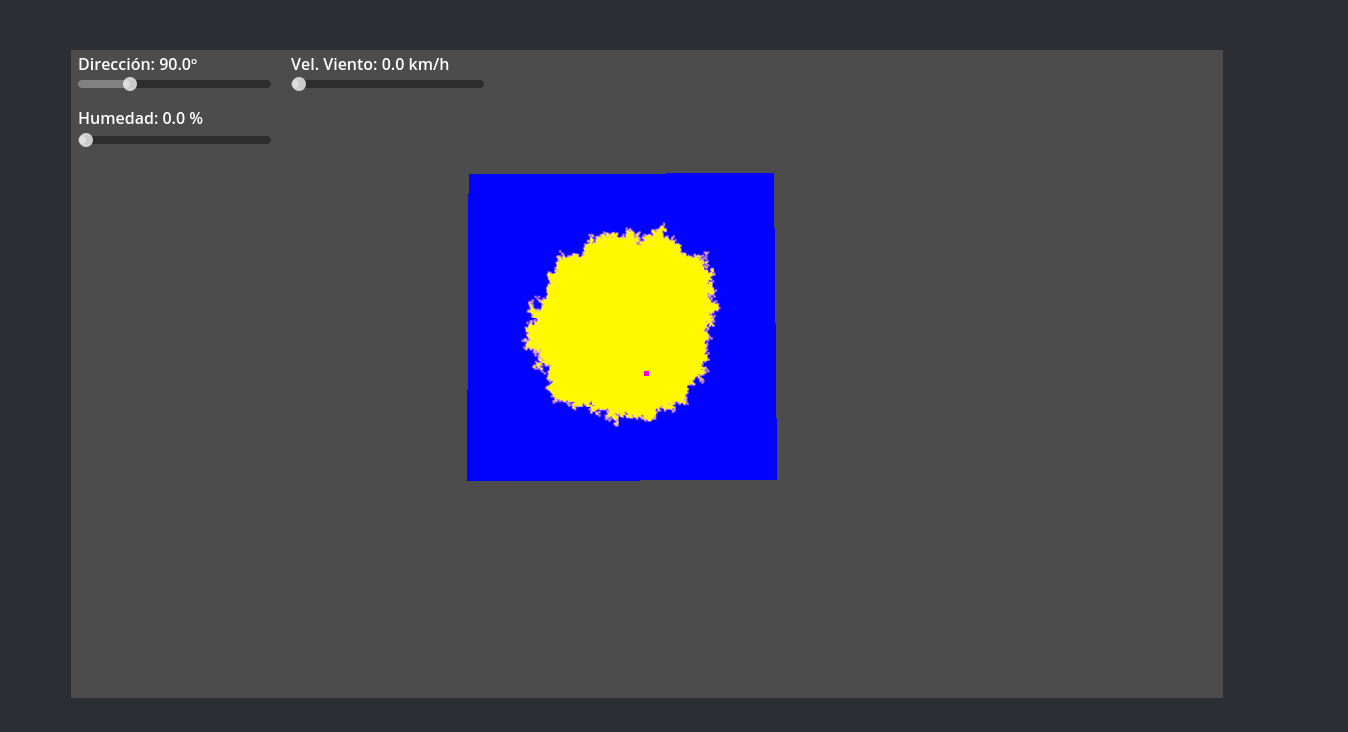
\includegraphics[width=0.7\textwidth]{imagenes/CasoEstudioA.png}
            \caption{Propagación isotrópica circular en terreno llano y sin viento.}
            \label{fig:validacion_base}
        \end{figure}

        \textbf{Resultado observado:} Cuando se desencadena el incendio en un punto con toda la vegetación homogénea y con ausencia de viento el modelo estocástico hace que el fuego se propague con una probabilidad muy parecida en todas las direcciones. El incendio dibuja un patrón de crecimiento circular a medida que avanza el tiempo de simulación. Esto valida que la matriz tridimensional del autómata no sufre de sesgos direccionales por la vecindad de Moore.\\


    \subsection{Caso de Estudio B: Influencia eólica y deformación elíptica}

        En el segundo escenario se mantiene un terreno plano con una combustible homogéneo de vegetación alta pero se introduce una variable meteorológica: rachas de viento constante a $40$ km/h incidiendo desde un ángulo fijo. \\

        \begin{figure}[H]
            \centering
            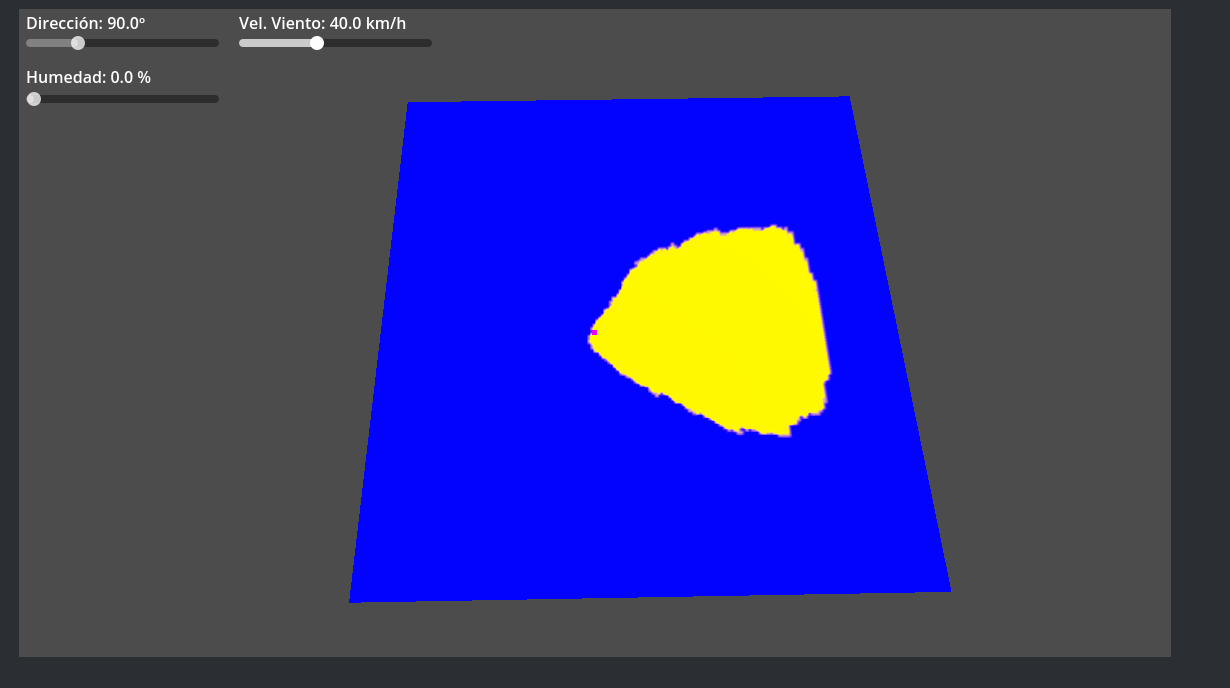
\includegraphics[width=0.7\textwidth]{imagenes/CasoEstudioB.png}
            \caption{Deformación elíptica del incendio bajo la influencia de viento fuerte unidireccional.}
            \label{fig:validacion_viento}
        \end{figure}

        \textbf{Análisis de resultados:} 
        Como se observa en la \textit{Figura X}, la simulación avanza de una manera realista siguiendo el factor del empuje del viento. El incendio deja de expandirse por igual en todas las direcciones y pasa a tener una deformación a favor de la dirección del aire que da como resultado una forma de elipse.
        
        Al observar el punto de ignición original (el extremo izquierdo de la superficie amarilla) se comprueban dos fenómenos que produce el modelo de Rothermel:        \begin{itemize}
            \item \textbf{Aceleración a favor del viento (Frente de avance):} En la dirección en la que sopla el viento la probabilidad de ignición aumenta propagándose en esa dirección con una mayor velocidad.

            \item \textbf{Estancamiento a contraviento (Fuego de retroceso):} El avance del fuego en contra de la dirección del viento es prácticamente nulo. Esto valida el correcto funcionamiento y la ecuación de Rothermel con respecto a la realidad.
        \end{itemize}

    \subsection{Caso de Estudio C: Influencia topográfica y convección}

        El tercer escenario evalúa el impacto del relieve, ignorando el viento. Se utiliza una geografía generada a partir de una textura de ruido con pronunciadas elevaciones y se realiza una prueba de doble ignición: el primer foco se inicia en la base de un barranco, y el segundo foco se establece en la cresta de una ladera.\\

        \begin{figure}[H]
            \centering
             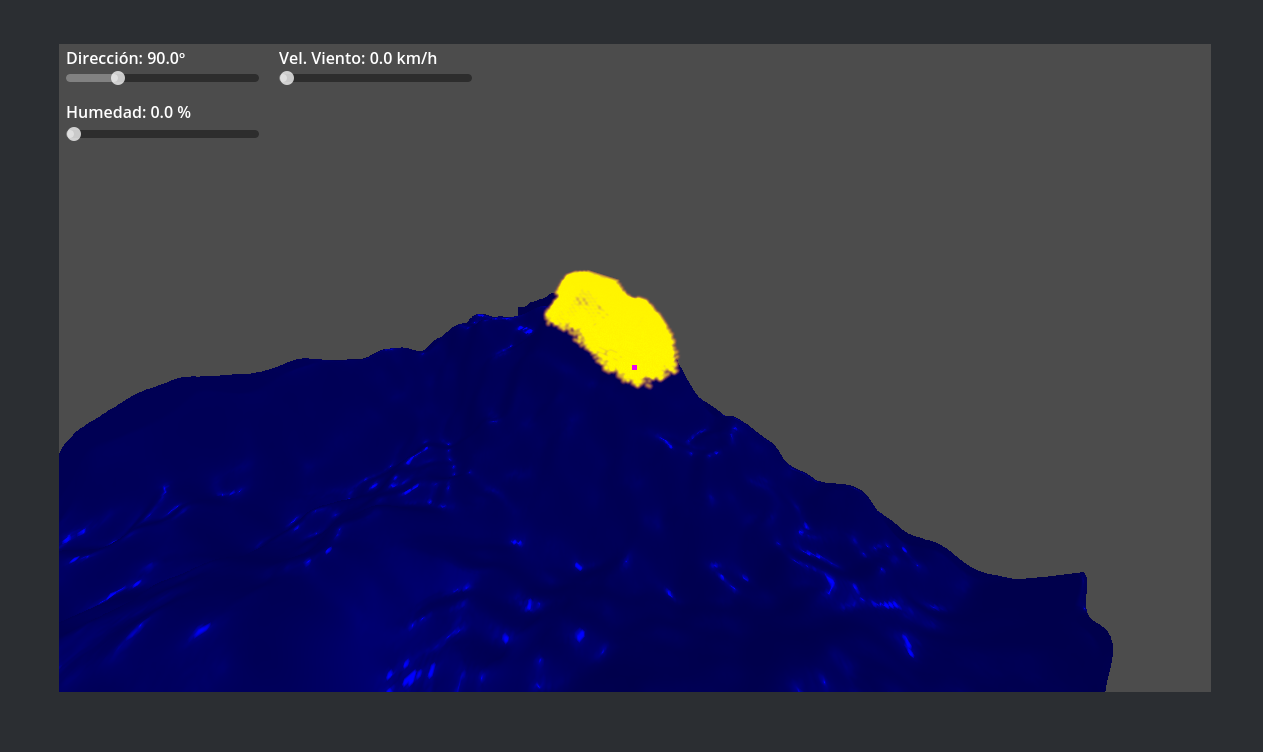
\includegraphics[width=0.7\textwidth]{imagenes/CasoEstudioC.png}
            \caption{Comportamiento convectivo: aceleración del fuego ladera arriba y estancamiento en el descenso.}
            \label{fig:validacion_topografia}
        \end{figure}

        \textbf{Resultado observado:} El simulador replica el comportamiento físico de la transferencia de calor por convección. Cuando se origina un foco en mitad de una ladera se propaga rápidamente a las zonas superiores, siguiendo el factor de inclinación del modelo de Rothermel, mientras que presenta una enorme dificultad para la propagación a zonas inferiores.

    \subsection{Conclusión de la Validación Física}

        El analisis de los tres casos de estudio confirma que la implementación en el  \textit{Compute Shader} de los factores probabilísticos de viento ($p_w$) y pendiente ($p_s$) son correctos. Como resultado se puede concluir que el simulador es capaz de ofrecer una representación orgánica y fiel a las físicas del fuego sin caer en el crecimiento artificial en forma de ciertos patrones propios de autómatas celulares mal calibrados.

